% !TEX program = xelatex
% Board meeting #1 Percolia -- vendredi 2 octobre 2026, 9h30-10h30 (visio Renater)
% Participants : Antoine Albrecht (Inria Startup Studio), Stéphanie Morales (Centre Inria d'Université Côte d'Azur),
%                Louis Hauseux, Alban Hauseux.
% Contenu : rétro-ingénierie du pitch deck « Percolia_PR_1.pdf » (septembre 2026), sauf la page de titre
%           (Board meeting #1) et le bloc « Conseil scientifique & réseau » (Josiane Zerubia) de la slide équipe.
% Thème : thème Inria de Presentation_Inria_Startup_Studio_2026-07-28 (dossier theme/ copié à l'identique).
% Compilation : make (XeLaTeX, comme le PDF d'origine).
\documentclass[A4,svgnames,10pt,aspectratio=169,usepdftitle=false]{beamer}

\usepackage[utf8]{inputenc}
\usepackage[french]{babel}
\usepackage{graphicx}

\title[Percolia]{\huge \textbf{PERCOLIA}}
\subtitle{\large Structuration automatique de données}
\date[2 octobre 2026]{Vendredi 2 octobre 2026}
\author[L. \& A. \textsc{Hauseux}]{%
   Louis \textsc{Hauseux} \& Alban \textsc{Hauseux} \\[4pt]
   \footnotesize \emph{Board meeting} \#1, avec Antoine \textsc{Albrecht} et Stéphanie \textsc{Morales}%
}
\institute{Inria Startup Studio}

% XeTeX ne fournit pas la primitive \draftmode (pdfTeX/LuaTeX), testée par le fond de page du thème
\ifdefined\draftmode\else\chardef\draftmode=0 \fi

\usetheme{inria}

% Logo Inria Startup Studio de la page de titre, à droite du bloc-marque RF-Inria
\newlength{\isslogowidth}

\hypersetup{
   allcolors   = rouge_inria,
   pdfauthor   = {Louis Hauseux \& Alban Hauseux},
   pdftitle    = {PERCOLIA - Board meeting \#1},
   pdfsubject  = {Board meeting \#1 Percolia - Inria Startup Studio - 2 octobre 2026},
   pdfkeywords = {Percolia, clustering, LiDAR, Inria, HGP-Clusterer, Board meeting}
}

\begin{document}

% Slide 1 : Page de titre
\begin{frame}
    \titlepage
    \setlength{\isslogowidth}{0.2\textwidth}%
    \begin{textblock*}{\isslogowidth}(\hmargin+\titlelogowidth+3.5mm,\vmargin-\titlelogovoffset)
        
\includegraphics[width=\isslogowidth]{imgs/Inria-StartupStudio-logo.png}
    \end{textblock*}
\end{frame}

% Slide 2 : Équipe fondatrice
\begin{frame}{Équipe fondatrice}
    \begin{columns}[T]
        \begin{column}{0.48\textwidth}
            \textbf{\bleu Louis Hauseux}
            \begin{itemize}
                \item Doctorat en informatique à Inria Sophia Antipolis.
                \item Normalien, double master en mathématiques fondamentales et appliquées.
                \item Conception et développement du noyau HGP-Clusterer.
            \end{itemize}
        \end{column}

        \begin{column}{0.48\textwidth}
            \textbf{\bleu Alban Hauseux}
            \begin{itemize}
                \item Ingénieur IMT Atlantique, master en ingénierie financière à Paris-Dauphine.
                \item Expérience en finance quantitative, audit et contrôle de modèles.
                \item Industrialisation, intégration client et développement commercial.
            \end{itemize}
        \end{column}
    \end{columns}

    \begin{block}{\normalsize Conseil scientifique \& réseau}
        \begin{itemize}
            \item \textbf{Josiane \textsc{Zerubia}} (Directrice de Recherche Inria, équipe \textsc{Ayana}).
        \end{itemize}
    \end{block}
\end{frame}

% Slide 3 : La limite des méthodes actuelles de clustering
\begin{frame}{La limite des méthodes actuelles de clustering}
    \textbf{\bleu Le standard : DBSCAN et HDBSCAN}
    \begin{itemize}
        \item Ces méthodes repèrent les zones denses, puis relient les points deux à deux.
        \item Elles sont rapides, disponibles dans les bibliothèques standards et très largement utilisées.
    \end{itemize}

    \vspace{0.25cm}
    \textbf{\bleu Le problème dans les scènes LiDAR réelles}
    \begin{itemize}
        \item Le bruit peut former un pont entre deux structures distinctes.
        \item L'algorithme finit alors par fusionner des objets qui devraient rester séparés. C'est l'effet de chaînage.
    \end{itemize}

    \vspace{0.25cm}
    \textbf{\orange Conséquence opérationnelle :} Mauvaise segmentation, anomalies mal isolées, résultats difficiles à exploiter, corrections manuelles.
\end{frame}

% Slide 4 : La rupture technique de Percolia
\begin{frame}{La rupture technique de Percolia}
    \textbf{\bleu HGP-Clusterer généralise le principe du Single-Linkage}
    \begin{itemize}
        \item Passage à l'ordre supérieur : les connexions ne sont plus évaluées entre deux points, mais à l'échelle d'un groupe.
        \item L'algorithme construit une hiérarchie de groupes à plusieurs échelles et retarde les fusions provoquées par le bruit.
    \end{itemize}

    \vspace{0.2cm}
    \begin{columns}[T]
        \begin{column}{0.48\textwidth}
            \textbf{\orange Propriétés du moteur}
            \begin{itemize}
                \item Sans entraînement ni données labellisées.
                \item Compatible avec des changements de capteur ou de domaine.
                \item Conçu pour de grands nuages de points.
            \end{itemize}
        \end{column}

        \begin{column}{0.48\textwidth}
            \textbf{\orange Spécificité industrielle}
            \begin{itemize}
                \item Des volumes, dimensions physiques ou modèles 3D peuvent guider la sélection des groupes.
                \item Le même moteur s'insère dans un pipeline existant sans réentraîner un modèle.
            \end{itemize}
        \end{column}
    \end{columns}

    \vfill
    {\scriptsize L. \textsc{Hauseux}, K. \textsc{Avrachenkov}, J. \textsc{Zerubia}, «~Generalization of Single-Linkage with higher-order interactions~», \emph{Applied Network Science}, 2026.}
\end{frame}

% Slide 5 : Le LiDAR comme premier marché
\begin{frame}{Le LiDAR comme premier marché}
    \begin{columns}[T,onlytextwidth]
        \begin{column}{0.8\textwidth}
            \textbf{\bleu Point d'entrée commercial}
            \begin{itemize}
                \item Jumeaux numériques, suivi d'actifs et inspection industrielle.
                \item Entreprises qui disposent déjà de scanners et d'un pipeline de traitement 3D.
                \item Scènes où le bruit et les objets imbriqués empêchent une séparation fiable.
            \end{itemize}

            \vspace{0.2cm}
            \textbf{\bleu Valeur mesurable}
            \begin{itemize}
                \item Moins de fusions erronées.
                \item Moins de correction manuelle.
                \item Une étape de traitement plus facilement automatisable.
            \end{itemize}
        \end{column}
    \end{columns}
\end{frame}

% Slide 6 : Exemple 1 : Détection d'anomalies de chantier (AIDetech)
\begin{frame}{\large Exemple 1 : Détection d'anomalies de chantier (AIDetech)}
    \small
    \begin{columns}[T,onlytextwidth]
        \begin{column}{0.53\textwidth}
            \textbf{\bleu Projet ISS de Marie Aspro avec Naval Group}
            \begin{itemize}
                \item \textbf{Objectif :} Détection automatique d'anomalies sur chantiers navals.
                \item \textbf{Données :} Confrontation entre un \textbf{modèle 3D théorique} (chantier attendu) et des \textbf{captations LiDAR} (chantier réel -- synthétique pour des besoins de confidentialité).
                \item \textbf{Collaboration Percolia :} Isoler les anomalies qui ne font pas partie du modèle théorique (ex. : casques de chantier, tuteurs, bâches).
            \end{itemize}
            \textbf{\bleu Le verrou}
            \begin{itemize}
                \item Nécessite un clustering assez fin prenant en compte le modèle 3D pour isoler proprement les anomalies de chantier.
            \end{itemize}
        \end{column}

        \begin{column}{0.43\textwidth}
            \centering
            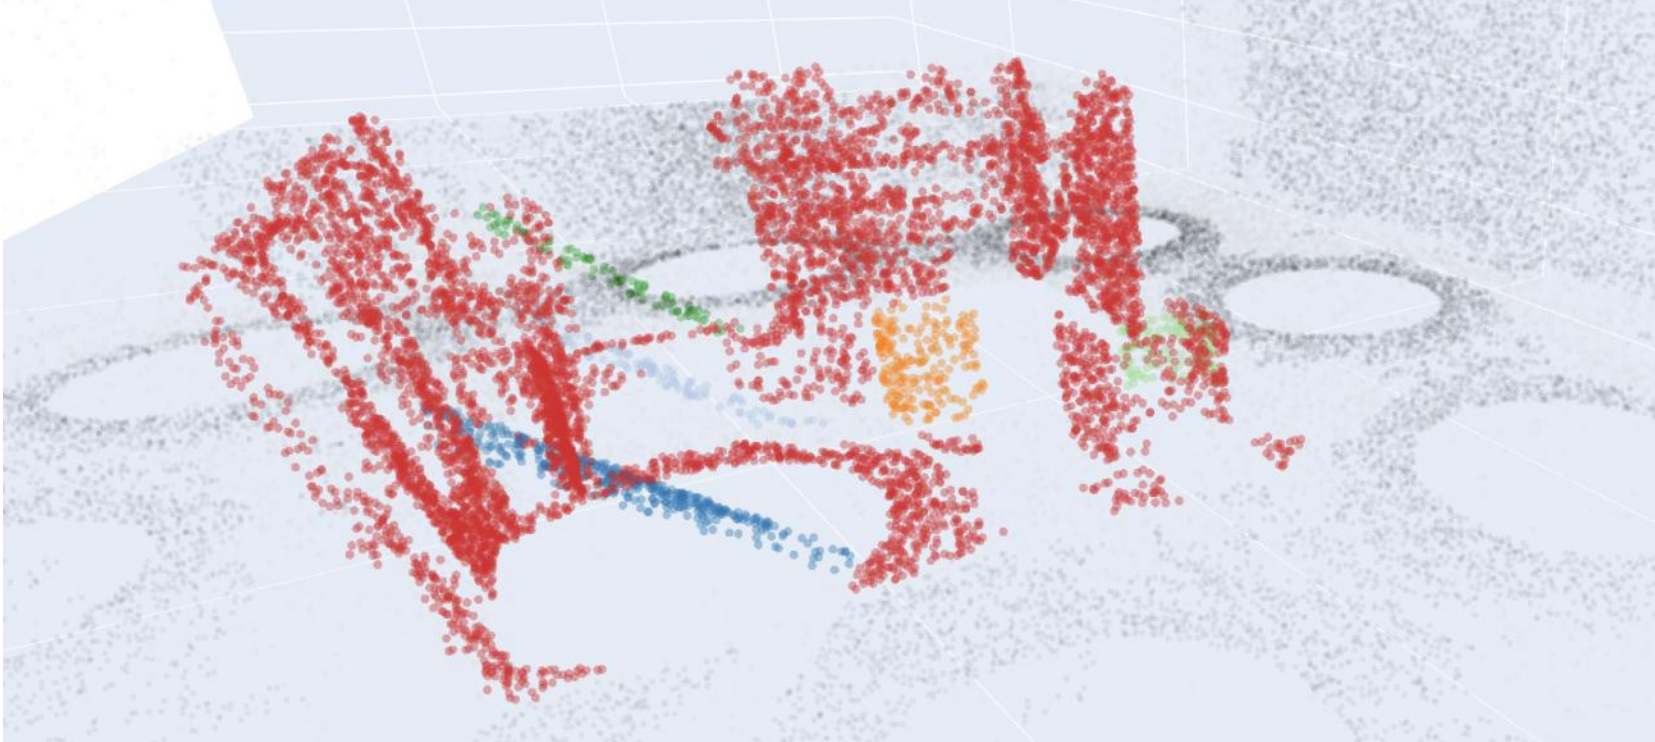
\includegraphics[width=\textwidth]{imgs/Resultat_MarieBenchmark.png}\\
            \tiny \textcolor{inria-2024-gris-bleu}{Détection des anomalies (cubes et tuteurs colorés) par rapport au modèle 3D (en rouge) sur le benchmark de Marie \textsc{Aspro}. © Marie \textsc{Aspro} / Naval Group.}
        \end{column}
    \end{columns}
\end{frame}

% Slide 7 : Du benchmark à la licence logicielle
\begin{frame}{Du benchmark à la licence logicielle}
    \begin{columns}[T]
        \begin{column}{0.5\textwidth}
            \textbf{\bleu 1. Benchmark ou pilote}
            \begin{itemize}
                \item Le client fournit quelques scans représentatifs.
                \item Percolia compare la qualité des groupes et le temps de calcul au pipeline existant.
            \end{itemize}

            \vspace{0.25cm}
            \textbf{\bleu 2. Intégration}
            \begin{itemize}
                \item Connexion aux formats du client.
                \item Configuration des contraintes géométriques ou du modèle 3D.
            \end{itemize}
        \end{column}

        \begin{column}{0.46\textwidth}
            \textbf{\orange 3. Revenu logiciel récurrent}
            \begin{itemize}
                \item Licence annuelle installée chez le client.
                \item API lorsque le cloud convient aux données et aux contraintes de sécurité.
            \end{itemize}
        \end{column}
    \end{columns}
\end{frame}

% Slide 8 : Trois voies d'accès au marché
\begin{frame}{Trois voies d'accès au marché}
    \begin{columns}[T]
        \begin{column}{0.31\textwidth}
            \textbf{\orange 1. Intégration}
            \begin{itemize}
                \item Benchmark, intégration, puis licence ou API.
                \item \href{https://www.greehill.com/}{Greehill}, \href{https://www.linkedin.com/company/ai-detech}{AI Detech}, \href{https://www.milla-group.com/}{Milla}, \href{https://www.hydroquebec.com/}{Hydro-Québec}.
            \end{itemize}
        \end{column}

        \begin{column}{0.31\textwidth}
            \textbf{\bleu 2. Constructeurs LiDAR}
            \begin{itemize}
                \item Notre moteur intégré au logiciel livré avec leurs scanners.
                \item \href{https://www.yellowscan.com/}{YellowScan}, \href{https://www.artec3d.com/}{Artec 3D}.
            \end{itemize}
        \end{column}

        \begin{column}{0.31\textwidth}
            \textbf{\bleu 3. Verticale complète}
            \begin{itemize}
                \item Percolia propose elle-même le service complet, de la donnée brute au résultat final.
            \end{itemize}
        \end{column}
    \end{columns}
\end{frame}

% Slide 9 : Au-delà du LiDAR
\begin{frame}{Au-delà du LiDAR}
    \textbf{\bleu Un moteur de clustering pour plusieurs familles de données}
    \begin{itemize}
        \item Le coeur mathématique travaille sur des données euclidiennes.
        \item Le nuage de points LiDAR constitue le premier produit commercial, avec un besoin industriel concret et observable.
    \end{itemize}

    \vspace{0.25cm}
    \textbf{\orange Applications possibles}
    \begin{itemize}
        \item Nuages de points et autres données euclidiennes.
        \item Vecteurs, embeddings et matrices de distances.
        \item Détection de communautés dans des graphes.
    \end{itemize}
\end{frame}

\end{document}
